\documentclass[11pt]{article}
\usepackage[english]{babel}
\usepackage[utf8x]{inputenc}
\usepackage{amsmath}
\usepackage{graphicx}
\usepackage[colorinlistoftodos]{todonotes}
\usepackage{indentfirst}
\usepackage{float}
\usepackage{hyperref}
\usepackage{array}

\begin{document}

\begin{titlepage}

\newcommand{\HRule}{\rule{\linewidth}{0.5mm}} % Defines a new command for the horizontal lines, change thickness here

\center % Center everything on the page
 
%----------------------------------------------------------------------------------------
%	HEADING SECTIONS
%----------------------------------------------------------------------------------------


\includegraphics[scale=.2]{logo.png}\\[1.5cm]
\textsc{\LARGE Advanced Operating Systems}\\[0.5cm]
\textsc{\Large Written Report}\\[0.5cm]
MAB2 Computer Science\\
2017-18

%----------------------------------------------------------------------------------------
%	TITLE SECTION
%----------------------------------------------------------------------------------------

\HRule \\[0.4cm]
{ \huge \bfseries Sparrow: Distributed, Low Latency Scheduling}\\[0.4cm] % Title of your document
by Kay \textsc{Ousterhout}, Patrick \textsc{Wendell}, Matei \textsc{Zaharia}, Ion \textsc{Stoica}\\
University of California, Berkeley
\HRule \\[1.5cm]
 
%----------------------------------------------------------------------------------------
%	AUTHOR SECTION
%----------------------------------------------------------------------------------------

\begin{minipage}{0.4\textwidth}
\begin{flushleft} \large
\emph{Author:}\\
Arman \textsc{Davidyan}
\end{flushleft}
\end{minipage}
~
\begin{minipage}{0.4\textwidth}
\begin{flushright} \large
\emph{Supervisor:} \\
Dr. Alain \textsc{Buys}
\end{flushright}
\end{minipage}\\[2cm]

% If you don't want a supervisor,
%uncomment the two lines below and remove the section above
%\Large \emph{Author:}\\
%John \textsc{Smith}\\[3cm] % Your name

%----------------------------------------------------------------------------------------
%	DATE SECTION
%----------------------------------------------------------------------------------------

{\large \today}\\[2cm] % Date, change the \today to a set date if you want to be precise

%----------------------------------------------------------------------------------------
%	LOGO SECTION
%----------------------------------------------------------------------------------------

%
\includegraphics[scale=.25]{logo.png}\\[1cm]
 
%----------------------------------------------------------------------------------------

\vfill % Fill the rest of the page with whitespace

\end{titlepage}


\section{Introduction}

	Nowadays, the Internet services become more and more interactive: instantaneous language translations, highly personalized searches etc. The clusters hosting these kinds of services need to be managed wisely to handle their workloads. This kind of jobs consists of many short and parallel tasks.\footnote{Note that every job is a set of tasks.} These tasks, usually, have a duration around 100ms length. When each task is only around hundreds of milliseconds long, the cluster scheduler will need to work at very high throughput: a large cluster scheduler, executing this kind of tasks, will need to do over one million scheduling decisions per second. Usually, a cluster scheduler is a centralized application that keeps the state of the whole cluster and manages the task assignment to the worker machines. This architecture is more suitable for high-performance computing, but it can be difficult to support high throughput workloads. This is the intention of Sparrow - a scheduler for low latency jobs.

    The first part of the report is an introduction to Sparrow. It will explain how Sparrow works and how well it performs in different scenarios. The second part of the job is a deepening in the subject of scheduling. It has two main topics: the first topic is an overview of the \textit{main architectures of cluster schedulers} and the second topic is a study of \textit{technics that can improve Sparrow}. The report will end with a brief overview of the impact that Sparrow had on the industry.

\section{Sparrow}

	Sparrow is a cluster scheduler, dedicated to jobs with short, low latency tasks. It was introduced in the article \textit{Sparrow: Distributed, Low Latency Scheduling}, in 2013, by the searchers from University of California, Berkeley.


	\subsection{Architecture}
    	\label{sparrowarchie}

		The main idea of the Sparrow is scheduling tasks in a completely decentralized way. Sparrow is a set of scheduling frameworks (see figure \ref{fig1}) that work independently - they do not exchange any information between each other. When a new job is submitted to the cluster, one of these frameworks will get to assign its tasks to the worker machines. All of the scheduling frameworks work the same way - they are instances of the same code. The exact way of assigning jobs to scheduling frameworks is not discussed in the article, but its implementation on GitHub shows that Sparrow uses a round-robin technic to distribute the jobs among its scheduling frameworks.
		
	\begin{figure}
		\centering
		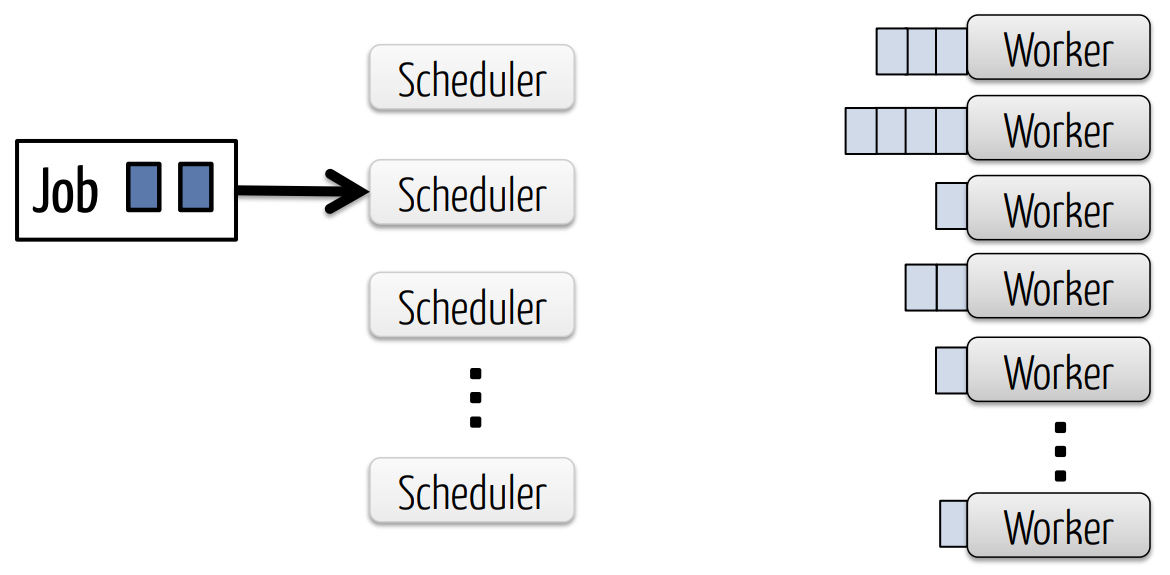
\includegraphics[scale=.25]{sparrow}
		\caption{The set of scheduling frameworks is Sparrow. Source: SOSP'13 talk on Sparrow.}
		\label{fig1}
	\end{figure}


	\subsection{Power of 2 choices}

		As it was stated, the set of scheduling frameworks that Sparrow consists of are instances of the same code. The main technique used in it is called \textit{power of 2 choices}. This is a technique that came from \cite{power}, an article about \textit{load balancing}. Load balancing is a problem of distributing $N$ tasks among $M$ resources, in the evenest way. In the aforementioned work, M. Mitzenmacher proves that if instead of randomly choosing a resource for a task, we have a choice between two random resources, the over-performance will be exponential.

		In some domains, this technique of assigning tasks to the best-suited resource, from a set of randomly chosen resources, could be a massive improvement over more complex techniques, because it has little overhead and can give good results. In Sparrow, the authors experimented to find out if this is the case in the domain of cluster schedulers. But the power of 2 choices is not the only technique used in Sparrow - there are some others that improve its overall performance.
        
        
    \subsection{Batch Sampling}
    	\label{batchsampling}
    
    	%TODO 13 issues
    	As it was stated, a job consists of some number of tasks, and power of 2 choices probes for each of this tasks individually two workers. This might not always return the best result. For example, if one has a job of two tasks, the probing for the first task could return 2 workers with 3 and 4 pending tasks respectively, and the probing for the second task could return workers with 1 and 2 pending tasks respectively. In this case, the first task will be placed on the worker with 3 tasks and the second task will be placed on the worker with 1 task. But intuitively, it will be more efficient to place the first task on the worker with 2 pending tasks. This is exactly what \textit{Batch Sampling} does. When a job with $N$ tasks arrive, $2N$ random workers will be probed at the same time, and the tasks will be placed on the $N$ least loaded workers. Figure \ref{fig2} visualizes this example.
    
    \begin{figure}
    		\hspace*{-.8in}
    		\centering
    		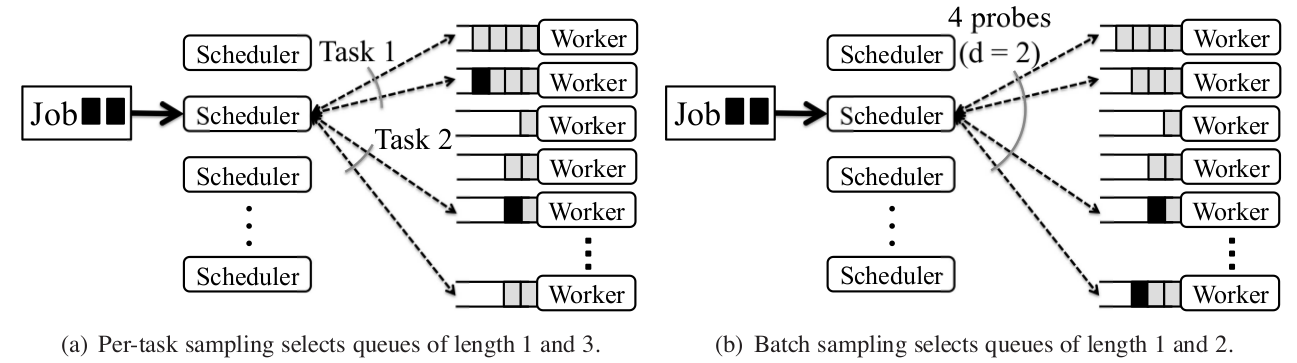
\includegraphics[scale=.35]{fig2}
    		\caption{Difference between power of 2 choices (par-task sampling) and power of 2 choices with batch sampling. Source: \cite{sparrow}}
    		\label{fig2}
    \end{figure}


    \subsection{Late Binding}
    
    	%TODO 18 issues
    	There is one major flaw in the batch sampling and power of 2 choices in general - the number of pending tasks is not a good indicator of the business of a worker. If we have two single-core workers, the first with 4 pending tasks and the second with 1 pending task, it does not always mean that it is better to place the new task on the worker with 1 task. If each of the 4 tasks will take 10 ms and the single task on the other worker takes 200 ms, then the first worker will be available to execute a task sooner. This is why many cluster schedulers use \textit{Late binding}. This is a technique that places reservations on $2N$ random workers for a job with $N$ tasks, instead of placing the task right away. When a worker is available to execute a reservation, it will notify the scheduler and the latter will send the task to the worker. This way, the tasks are assigned to the workers that are available first. When all the tasks are assigned to the fastest $N$ workers, the other $N$ workers will get a message to forget about their reservations.


    \subsection{Experiments}
    
    	%TODO 8 issues
    	To test the efficiency of Sparrow, the authors performed some number of tests. Some of them are completely analytic, which means no tests on hardware were done, and some are practical. Among practical experiments, they performed 2 kinds of tests: with real-world workloads and with synthetic workloads. A synthetic job is a job that contains tasks that ask the worker machine to sleep one of its core for some time. All the practical experiments have been performed on a cluster of 110 machines. To perform the experiments, Sparrow was integrated into the Apache Spark cluster framework (it replaced Spark's native scheduler).


		\subsubsection*{Theoretical Analysis}
			\label{theoreticalanalysis}
        
        	The authors did only one theoretical study of Sparrow. The point of this study was to discover the probability for a job to experience a zero wait time \textit{i.e.} the probability for all task of a job to be placed on idle machines.
            
            \begin{table}
            	\caption{$\rho$ is the cluster load and m is the number of tasks in a job.}	
            		\centering
                \begin{tabular}{ | l | l |}
                    \hline
                    Random Placement & $(1-\rho)^m$  \\ \hline
                    Power of 2 choices & $(1-\rho^2)^m$  \\ \hline
                    Sparrow & $\sum_{i=m}^{2*m}(1-\rho)^i$$\rho^{2*m-i}$${2*m}\choose{i}$ \\
                    \hline
                \end{tabular}
        	\end{table}
            
            In the table above, one can see the probabilities for 3 different techniques to place all tasks of some job on idle workers, in a cluster with single core machines. The authors varied the cluster load from 0 to 1, to obtain the graph in figure 3. It shows that the theoretical probability of Sparrow to place all task on idle machines is very close to 1 when the cluster load is lower than 0.5 and it is very close to 0 when it is higher than 0.5.
            
            \begin{figure}
            		\centering
            		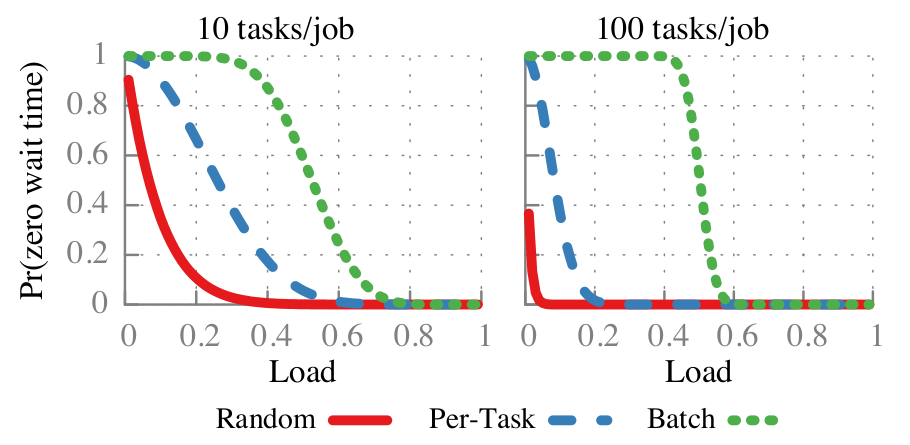
\includegraphics[scale=.3]{fig3}
            		\caption{Theoretical probability of Sparrow placing the tasks on idle machines. Because of the fact that we analyze the probability of placing tasks on idle machines, Sparrow will not use the late binding, hence it will be as good as batch sampling.}
            		\label{fig3}
            \end{figure}
         
         	%TODO 6 issues   
            The authors also performed the same test on a cluster with 4 core machines. They added an additional constrains to avoid ``gold rush effect'': because of the fact the decentralized schedulers in Sparrow does not share any information between each other, if two of them find the same idle worker at the same time, both will place 4 tasks on that worker; hence, there will be 4 tasks that will experience an unexpected delay. To avoid this problem, Sparrow let each scheduler to place only one task on a single worker. The result of this experiment is that 79.9\% of jobs will be placed on idle workers at 80\% workload.
            
            
        \subsubsection*{Experiment with TPC-H}
        
        	Another experiment that authors performed was executing queries of TPC-H benchmark on a cluster scheduled by Sparrow. TPC-H\footnote{TPC-H stands for Transaction Processing Council Ad-hoc/decision support benchmark} is a benchmark frequently used for testing the performances of database software. It contains sets of queries that are inspired by real-world scenarios.
            
            %TODO 9 issues
            The authors composed 4 different sets of queries: the first set keeps the cluster load at 80\%, the second set contains the jobs that have two groups of tasks that can not be processed in parallel, the third set contains the jobs with tasks of various durations, and the fourth set contains jobs with tasks that have different constraints.
            
            The result of this experiment shows that, on average, Sparrow performs only 12\% worse than the ideal scheduler. The performance of the ideal scheduler is computed by supposing that it always places the tasks on idle workers (no task is queued, no job experiences any waiting time). In other words, the execution time of a job, scheduled with the ideal scheduler, is equal to the longest, non-parallel, sequence of tasks in it.
            
            \begin{figure}
            		\centering
            		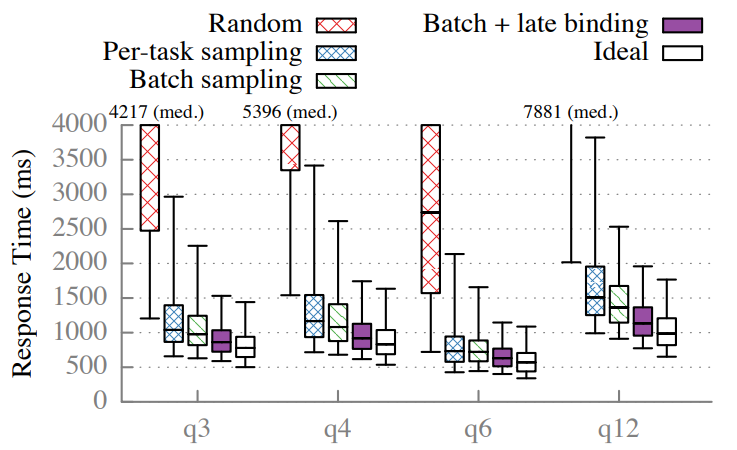
\includegraphics[scale=.35]{fig4}
				\caption{q3, q4, q6, and q12 are respectively the first, the second, the third and the fourth sets.}            		
            		\label{fig4}
            \end{figure}
        
        
        \subsubsection*{Experiment with a scheduler's fail}
        
        	%TODO 6 issues
        	Any of the simplistic scheduling frameworks of Sparrow can fail. In the case of a failure, it is necessary to be sure that the jobs assigned to the failed framework will be executed. For this purpose, each of them is launched with a list of backup scheduling frameworks, and Sparrow verifies every 100 ms that they are functional. If one of the frameworks fails, Sparrow will assign his jobs to the first framework in the backup list (of the failed scheduling framework). The intermediate progress of a job acquired before the failure will be lost. The experiment that authors performed showed that it takes 120 ms for Sparrow to detect and reassign the tasks of a failed framework. Because of the fact that Sparrow is dealing with short tasks, only a few jobs will be penalized because of the framework failure.
        
        
        \subsubsection*{Sparrow compared to a centralized scheduler}
        
        	In a case of a centralized scheduler, all the scheduling decisions are made by a single agent. Because of it, this kind of schedulers is more convenient for High-Performance Computing. To prove this, the authors compared the performance of Sparrow with the performance of Sparks native centralized scheduler on a cluster at 80\% workload. The experiment showed that when the duration of the tasks are 1.3 second or less, the Spark's native scheduler is no longer able to work properly and experience infinite queuing, while Sparrow is able to correctly schedule for tasks of any duration.
        
        
        \subsubsection*{Sharing a cluster between multiple users}
        
        	%TODO 6 issues
        	To analyze how fairly Sparrow is capable to share a cluster between different users, the authors performed an experiment with a cluster shared between two users. The first user always requires as many resources as possible from Sparrow all the time during the experiment. The second user requires no resources at all for ten seconds; then he requires 25\% of the cluster capacities for another 10 second; then he requires 50\% of the cluster capacities for another 10 seconds; then he requires only 25\% of the capacities for another 10 seconds; for the last 10 second interval, the second user requires no resources at all.
            
            %TODO 6 issues
            The result of this experiment showed that Sparrow is able to fairly share the cluster between different users, but sometimes the cluster may be used not at the maximum of its capacities. The reason of this problem is related of the decentralized nature of Sparrow - it contains many scheduling frameworks that are not inter-connected, hence, they don't have the complete image of the cluster utilization by users. Figure \ref{fig5} illustrates the experiment.
            
            \begin{figure}
            		\centering
            		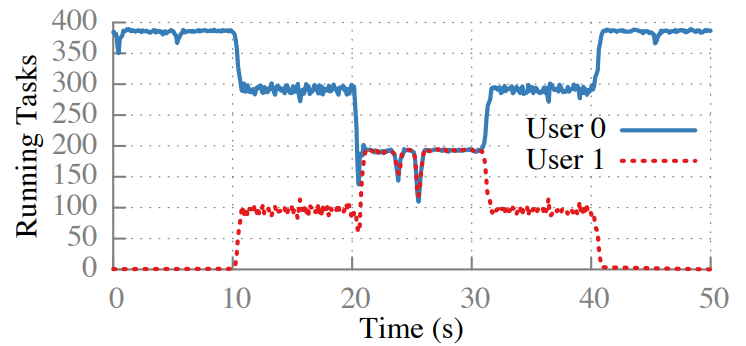
\includegraphics[scale=.35]{fig5}
            		\caption{Sparrow shares the cluster between two users.}
            		\label{fig5}
            \end{figure}
        
        
        \subsubsection*{Shielding high priority tasks from low priority tasks}
        	 \label{preemption}
        	
        	%TODO 6 issues
            An important aspect of Sparrow is protecting high priority users from low priority users. To do so, the authors implemented Sparrow in the following way: each worker machine has many queues - each of them contains only tasks with the same priority and no node has two queues with the tasks of the same priority. When a worker is ready to execute a new task, he will pull a task from the highest non-empty queue.
            
            %TODO 5 issues
            In this experiment, the authors kept the proportion of the high priority load at 25\% of the cluster capacities and varied the proportion of low priority load. The experiment showed that Sparrow is able to protect the high priority tasks from low priority task when the total cluster load is less than 100\%. But, when the total cluster load is at 100\% or more, the high priority get 40\% worse execution time. The table below shows the complete results of the experiment.
            
            \begin{table}
				\caption{HP stands for high priority workload, LP stands for low priority workload, the values outside the parentheses are the median response times and the values inside the parentheses are the 95th percentile response times.}
				\centering
                \begin{tabular}{ | c | c | c | c |}
                    \hline
                    HP load & LP load & HP response time in ms & LP response time in ms  \\ \hline
                    0.25 & 0 & 106(111) & N/A  \\ \hline
                    0.25 & 0.25 & 108(114) & 108(115) \\ \hline
                    0.25 & 0.5 & 110(148) & 110(449) \\ \hline
                    0.25 & 0.75 & 136(170) & 40.2k(46.2k) \\ \hline
                    0.25 & 1.75 & 141(226) & 255k(270k) \\
                    \hline
                \end{tabular}
        	\end{table}
        	
        
        \subsubsection*{Why power of 2}
        	\label{probingratio}
        
        	%TODO 9 issues
        Another interesting point for authors was to find out if the probing ratio of 2 is the best choice or it is better to have a higher or lower probing ratio. To answer that question, the authors performed two experiments where they varied the probing ratio at constant the cluster load. The first experiment kept the cluster load at 80\% and the second one kept it at 90\%. The range of probing ratio was between 1.0 (1 probing par task \textit{i.e.} random placement) to 3 (3 probings par task). The experiments showed that the best probing ratios are 1.5 and 2 because if the probing ratio is lower, the scheduling frameworks are not able to find idle workers, and if the probing ratio is higher, there is too much message exchange in the cluster and that also delays the probing decision. The authors choose the probing ratio of 2 because it is easier to have an integral probing ratio. The result of the experiment is in figure \ref{fig6}.
        
        \begin{figure}
        		\centering
        		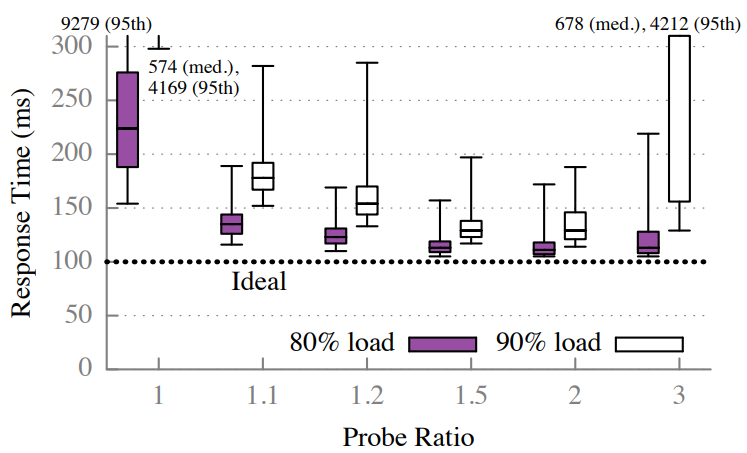
\includegraphics[scale=.35]{fig6}
        		\caption{Effect of probe ratio on job response time at two different cluster loads. Whiskers depict 5th and 95th percentiles; boxes depict median, 25th, and 75th percentiles}
        		\label{fig6}
        \end{figure}


\section{Main architecture of cluster scheduling}

	The authors of Sparrow adapted a specific architecture for the process of scheduling tasks. To better understand the choices they made during implementing Sparrow, it will be useful to take a look at mainstream cluster scheduler.
    
    %TODO remove the explanation of schedulers? If not fix, the paragraph
	Every major company adapts its cluster scheduler to its needs, but basically, one can divide them into five large categories: monolithic, two-level, shared state, fully-distributed, and hybrid. %Monolithic architecture is the most popular. A scheduler of this type is using a centralized algorithm for all jobs. For example, Borg, created and used at Google, is a monolithic scheduler. Two-level schedulers have a single resource manager and much parallel scheduling (like Sparrow). The parallel schedulers are not necessarily homogeneous, and the single resource manager shares the resources between them. Mesos \cite{mesos} is an example of this kind of scheduler. In the case of shared state schedulers, there are many parallel, not necessarily homogeneous, scheduling frameworks. Each of the schedulers has a complete view of the cluster load, and there are no direct interactions between schedulers. Omega \cite{omega} is an example of shared state cluster. The architecture of shared state clusters is the closest, among the 3 aforementioned architectures, to the architecture of Sparrow. Figure 1 illustrates an overview of the three architectures.
    
    \begin{figure}
    		\centering
    	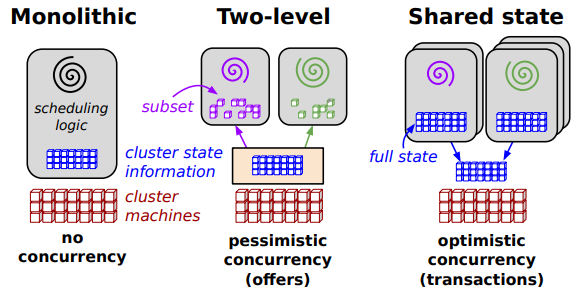
\includegraphics[scale=.5]{architectures}
        \caption{An overview of the most popular scheduling architectures. Source: \cite{omega}. Because of the fact that \cite{omega} discusses only monolithic, two-level and shared states scheduling techniques, the fully-distributed and hybrid scheduling techniques are not illustrated.}
    \end{figure}

	\subsection{Monolithic scheduling}
    
    	%TODO add Borg story when developers use side effects
        Monolithic schedulers are the most popular cluster schedulers. They have a central agent that performs all scheduling decisions and sees the cluster resources as a single entity. This approach is most suited for high-performance computing because in HPC we worry less about the speed of execution than in modern clusters. 
        
        Usually, the centralized agent is a complicated algorithm because it must contain all the policies and constraints of the system. Also, the scheduling algorithm gets updated over time which leads to a very complicated code base, and difficulties for future updates. But the most dangerous situation that can be faced with a monolithic scheduler is the side effects. When the code gets complicated, a lot of undocumented side effects appear, and the developers tend to use them in order to optimize their programs. The problem is that once the code of the scheduler is changed, some side effects can disappear and the programs using them will no longer work.
        
        %TODO 10 issues
        The central agent contains all the necessary functions to compute the priority of a task. After the priority is computed, all tasks are ordered by their priority and the execution will start by the tasks in the head of the list. Some schedulers support code paths with the jobs. In this case, the actor that submits the job can also submit a path to a code that the scheduler will execute in order to find the priority of a task. In this way, the standard policies of the scheduler can be overridden for certain jobs.
        
       %NOTE add statically partitioned schedulers
       
	\subsection{Two-level scheduling}
    
    	This type of scheduling was first introduced by Mesos \cite{mesos}. Two-level schedulers have a single resource manager, but many scheduling frameworks. The purpose of the resource manager is dynamically defining the resources for each scheduler. The manager offers to the scheduler only the resources that are currently unused, and any resource is offered only to one scheduling framework at a time, to avoid conflicts. An important goal of the resource manager is to share the resources fairly between frameworks. YARN, another two-level scheduler used in Apache Hadoop\footnote{Hadoop is an open-source framework that allows processing large data sets across a cluster of computers}, lets the scheduling frameworks to ask from resource manager the resources it needs, instead of waiting for an offer.
        
        The scheduling frameworks in the two-level schedulers can be heterogeneous. This means that each framework can target only some particular type of jobs. This distinction between different frameworks can be based on the duration of tasks, the parallelism of tasks in a job, some constraints of the job etc. The scheduling frameworks have only access to a part of the cluster and do not see the state of the whole cluster. Because of this fact, the gang scheduling (more on this in \ref{gang}) might be difficult to implement (because some tasks can require different types of resources, and all the tasks must be executed at once). Some schedulers as Mesos \cite{mesos} can let its scheduling frameworks to accumulate resources needed for a gang scheduling, but this might lead to deadlocks.
    
    \subsection{Shared state scheduling}

		A shared state scheduler contains many scheduling frameworks, but no resource manager. The frameworks can be heterogeneous and need to compete with each other to obtain a resource. Each framework contains a replica of the cluster state. If one framework wants to request some resource, it should update its local replica and will send the information about the request to other frameworks. The request may fail if another framework requests the same resource in the meantime. Usually, the scheduling is done in an incremental manner - a framework occupies all non-conflicting resources. Although to perform gang scheduling (all task executed at the same time, or none), a framework can do atomic request - all resources or nothing. Examples of his king of scheduling are Omega \cite{omega} by Google and Apollo \cite{apollo} by Microsoft.
    
    \subsection{Fully-distributed scheduling}
    	%TODO has distributed scheduling gain any popularity?
    	This kind of scheduling is similar to shared state scheduling, except that the scheduling frameworks don't interact with each other. The schedulers compete with each other to obtain the resources. As Sparrow is an example of a fully-distributed scheduler. A more detailed explanation of this kind of scheduling can be found in \ref{sparrowarchie}.%TODO talk about the disadvantages of fully-distributed scheduling?
        
    \subsection{Hybrid scheduling}
    
        A hybrid scheduler adapts two or more techniques at once. For example, we can combine the techniques of monolithic scheduling and fully-distributed scheduling. A hybrid of this kind should have a central algorithm that decides how a job should be scheduled; if the tasks are short and can be executed in parallel, the job can be scheduled under fully-distributed scheduling technique, otherwise, it should be scheduled by the monolithic scheduler.


\section{Possible improuvements}

	Sparrow is very simplistic cluster scheduler - the only techniques it adapts are the power of 2 choices, batch sampling, late binding and proactive cancelation. The authors of Sparrow realized that, and during the work, they mentioned on multiple occasions that it needs improvements. They even provided a list of techniques \cite[section 8]{sparrow} that are used in different schedulers and can improve Sparrow. Unfortunately, they were brief in explanation. It would be useful to dig deeper into this subject to see what are these techniques and understand if they are possible to implement in Sparrow.
	
	\subsection{Preemptive scheduling}
	
		Preemption is the process of interrupting a task that is currently executing, in favor of a new task with higher priority that has just arrived. Preemptive scheduling is one technique that is implemented for most of the schedulers, but not for Sparrow. In \cite[subsection 7.8]{sparrow}, also explained in \ref{preemption}, the authors of Sparrow studied the effect of low priority tasks that are abusing the resources of the cluster and not letting the high priority tasks to be executed in time. In the experiment, only 25\% of the cluster load was high priority tasks, hence, they could be, and they should be, executed in time. But, because of the overpressure of low priority tasks, they get 40 \% worse execution time in average. If Sparrow had preemption, the scheduling frameworks could have interrupted some low priority tasks in favor of high priority tasks, and the important job would have shorter execution times
		
		Preemptive scheduling seems to be fairly easy to implement in Sparrow. For recall, Sparrow keeps $N$ priority queues on each working machines; each of these queues is dedicated to tasks of only one level of priority; when a new slot is empty, the worker is going to take the first reservation from the highest priority queue. If we implement preemption in Sparrow, then, each time a worker gets a new reservation, it should verify if the task in execution (or one of the tasks in the execution) has lower priority than the new task. If it is the case, the high priority task can be placed in the slot of the low priority task, and the latter should be placed back in his queue (or in a queue with higher priority to make sure it will not be paused again in the future).
		
		The only problem related to preemption is the \textit{context switching}. Context switching is the process of saving the state of a process (or task) in the memory until the moment its execution can be resumed, from the point where it was paused. Context switching is needed when a new process with a higher priority needs to take the place of the process that is currently executing and is not finished yet. The fact of saving the context of the paused process (storing its current state and all its variables) and then reloading it when the process should be continued leads to wasted CPU time. The problem Sparrow can face is the rightfulness of the context switching. It is possible that is some scenarios (for example when current task is very short or close to its end), it would be more preferable to let the current low priority task to finish. It is an important problem because Sparrow is a scheduler for short, low latency tasks.
		
		Another limitation of preemption for Sparrow is its decentralized nature. If one worker pauses the execution of a task, he can not pass it to another worker that is free. This leads to the fact that low priority tasks might get large delays. Also, after implementing the preemption scheduling, additional experiments should be made (and some experiment should be redone), to understand how the preemption affected the overall performance of Sparrow. It is possible that it will worsen the average task duration. If it is the case, the authors should make a choice between preemption and overall performance.
		
		
	\subsection{Inter-job constrains}
	
		Inter-job constraints let the owner of a job, force some additional constraints on the worker machines where the tasks of the job are going to be executed. For example, a user A can forbid the scheduler to assign his jobs to worker machines where some particular user B's jobs are executing. Because of the fact that Sparrow's scheduling frameworks work independently, it is not possible to force this kind of constraints. The authors say that inter-job constraints will require considerable modification of Sparrow code base \cite[section 8]{sparrow}, but there might be a way of implementing it with no major modifications.
		
		To implement inter-job constraints of type ``tasks of user A should not be executed with tasks of user B'', sparrow can add an additional queue on each worker machine. A scheduling framework can ask the scheduler to place the reservations for some tasks to this special queue. The worker machines should execute the tasks from this queue only when no other tasks from any other queue is executing. If all slots of a worker machine execute the tasks from the same job, it is obvious that one job tasks will not be executed along with any other job tasks. This implementation may require some changes not only in the functioning of working machines but also in the way how scheduling framework place their tasks on workers. The reason of this is the constraints that the authors forced to the scheduler \cite[section 5]{sparrow}: no scheduling framework should place more than one task on a single working machine, to avoid the gold rush effect.
		
		In the case, if two jobs, A and B, should be executed on the same machine, the agent, that assigns the jobs to the scheduling frameworks, can merge these two jobs into one and the framework should place the tasks on the same worker.
		
		This is just one possible implementation of inter-job constraints that seems to be possible, and do not need major changes in the Sparrow code base. Although, this solution does change some aspects of job assignment to the workers. And again, this implementation might slow down the performance of Sparrow, and needs to be well tested.
		
		Another implementation of inter-job constraints could be allowing message interactions between workers machines and scheduling frameworks to find out if some constraints can be respected before assigning jobs. But the problem with this solution is that in \cite[subsection 7.9]{sparrow} (also explained in \ref{probingratio}) if we increase the probing ration, the performance of Sparrow drops because workers spend too much time in exchanging messages. Hence, most likely, increasing message exchanges for inter-job constraints support will also affect the performance of Sparrow.

	\subsection{Gang scheduling}
		\label{gang}
	
		Gang scheduling is a technique when some (or even all) tasks of a job are executed at the same time. Usually, this kind of scheduling is needed when different tasks need to communicate with each other during their execution. If these kind of tasks are not in execution in the same time, then, from time to time, some of them should be put into sleep while they wait until the moment when needed tasks can respond. If these tasks are not executed in parallel, a heavy overhead can be present because of constant context switching.
		
		The authors \cite[section 8]{sparrow} suggest that gang scheduling could be implemented using the bin packing problem. It is a mathematical problem of minimizing the number of bins we need to place a finite number of objects into them. As it was explained \ref{batchsampling}, Sparrow uses batch sampling to find the $N$ list loaded worker machines to place tasks on them. Whilst it happens often that tasks are placed on idle machines \ref{theoreticalanalysis}, it is not guaranteed. To truly implement gang scheduling, the scheduler needs a central agent that has a view of the whole cluster. But implementing such kind of agent opposes to the principal idea of Sparrow. It will be difficult to implement gang scheduling in a decentralized scheduler like Sparrow.
		
		One naive way of implementing it would be using preemption. If the tasks that should be gang-scheduled are given very high priority, the worker machines will pause currently executing tasks (if needed) to execute the new tasks in a gang. The only problem is that by doing so, we will have an overhead related to context switching for paused tasks, and avoiding the context switching is the initial reason to implement gang scheduling. Also, in this situation, if two gangs are overlapped, the second gang can interrupt the execution of the first gang, and, again, this will lead to overhead because of context switching.
		
		%TODO Query-level policies
		
	\subsection{Worker failures}
	
		The scheduling frameworks are regularly probed every 100 ms to find if one of them has failed, but the failures of worker machines are not tracked at all. In the case, if a worker fails, the frameworks will not know if it is functioning. If during batch sampling, $m$ worker machines fail, the scheduling framework will probe only $2N - m$ worker machines, without knowing. Also, another problem with worker machine failure is what happens to the tasks that were executing during the failure - all the progress is lost and the tasks should be restarted.
		
		The worker failure control can be implemented in a centralized way, like scheduler failure control. The authors think that the best solution is to have a centralized agent that verifies the functioning of the worker machines, and places the failed worker in a soft state list. The framework should periodically check the list so that they do not probe failed workers.
		
		The \textit{soft state} is a term usually used in networking. It means a list that is regularly cleared after a fixed period of time. In the case of worker failures, the list will contain the workers that are failed; once every $n$ ms, the list is emptied - if a worker is still unavailable, it should be placed again in the list; normally, $n$ should be equal to the time the central agent needs to detect and relaunch a failed worker.
	
	\subsection{Dinamically adapting probing ratio}
	
		In the \cite[subsection 7.9]{sparrow} (also explained in \ref{preemption}), the authors already studied the effect of probing ratio. The experiment concluded that if we have a small probing ratio, it is difficult for scheduling frameworks to find lightly loaded machines and if the probing ratio is large, there are too many message exchanges between worker and scheduling frameworks - this leads to overhead and delays the speed of decision making. But this experiment was done only twice, once with 80\% cluster load and once with 90\% cluster load. These are very high cluster loads, and the cluster load is going to be variable. Moreover, \textit{Reiss and al} \cite{hetero} claim that the overall CPU usage of Google clusters does not exceed 60 \% (figure \ref{google}). Hence, it is possible that having a constant probing ratio of 2 is not the best solution.
		
		\begin{figure}
			\centering
			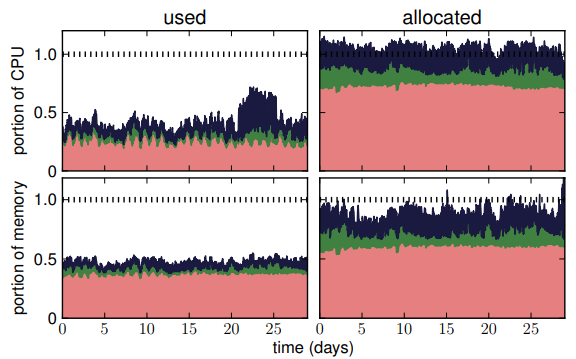
\includegraphics[scale=.5]{google}
			\caption{Moving hourly average of CPU (top) and memory (bottom) utilization (left) and resource requests (right). The dashed line near the top of each plot shows the total capacity of the cluster. Source: \cite{hetero}}
			\label{google}
		\end{figure}
		
		It might be possible to achieve better results by adjusting the probing ratio to the cluster load. If the cluster load is low, the schedulers could do more probes to be more successful in finding lightly loaded machines; if the cluster is highly loaded, the probing ratio should decrease to reduce the messaging overhead in the system. Obviously, it would require to find out experimentally the equation that adapts the probing ration the best, depending on the cluster load.
		
		The main difficulty of dynamically adapting the probing ratio is the decentralism of Sparrow - to adapt the probing ratio to the cluster load, Sparrow needs to determine this load. It would require to implement some mechanism that will keep track of the workers' load and tasks that are still to schedule. This mechanism may considerably change the architecture of Sparrow and will need a practical testing.
		




\begin{thebibliography}{9}

\bibitem{sparrow}
  K. Ousterhout, P. Wendell, M. Zaharia, and I. Stoica,
  \textit{Sparrow: Distributed, Low Latency Scheduling},
  In Proceedings of SOSP '13,
  Pages 69-84 ,
  2013.

\bibitem{github}
  K. Ousterhout, P. Wendell, M. Zaharia, and I. Stoica,
  \textit{Official Github repository of Sparrow},
  \url{https://github.com/radlab/sparrow},
  [Online; accessed June 2018].

\bibitem{power}
  M. Mitzenmacher
  \textit{The Power of Two Choices in Randomized Load Balancing}
  IEEE Transactions on Parallel and Distributed Systems,
  Volume 12,
  Issue 10,
  October 2001.

\bibitem{omega}
  M. Schwarzkopf, A. Konwinski, M. Abd-El-Malek, and J. Wilkes,
  \textit{Sparrow: Distributed, Low Latency Scheduling},
  EuroSys '13,
  Pages 351-364,
  2013.
  
\bibitem{mesos}
  B. Hindman, A. Konwinski, M. Zaharia, A. Ghodsi, A. D. Joseph, Randy Katz, Scott Shenker, and I. Stoica,
  \textit{Mesos: A Platform for Fine-Grained Resource Sharing in the Data Center},
  In Proceedings of NSDI'11,
  Pages 295-308,
  2011.
  
\bibitem{borg}
  A. Verma, L. Pedrosa, and M. Korupolu,
  \textit{Large-scale cluster management at Google with Borg},
  In Proceedings of EuroSys '15,
  Article No. 18,
  2015.

\bibitem{apollo}
  E. Boutin, J. Ekanayake, W. Lin, B. Shi, J. Zhou, Z. Qian, M. Wu, and L. Zho,
  \textit{Apollo: Scalable and Coordinated Scheduling for Cloud-Scale Computing},
  In Proceedings of OSDI' 14,
  Pages 285-300,
  2014.
  
\bibitem{hetero}
  C. Reiss, A. Tumanov, G. R. Ganger, R. H. Katz, and M. A. Kozuch
  \textit{Heterogeneity and dynamicity of clouds at scale: Google trace analysis},
  In Proceedings of SoCC,
  Article No. 7,
  2012.


\end{thebibliography}

\end{document}



























